\begin{frame}{Vision-Based Robotic Grasping of Diverse Objects}{}
    \begin{columns}%
        \begin{column}{0.5\textwidth}%
            \centering
            \hspace{-0.5cm}
            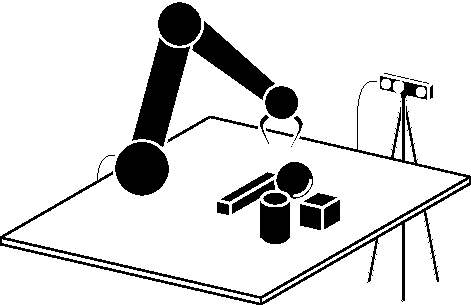
\includegraphics[height=4.75cm]{graphics/setup_sketch.pdf}
        \end{column}
        %
        \begin{column}{0.5\textwidth}%
            \centering
            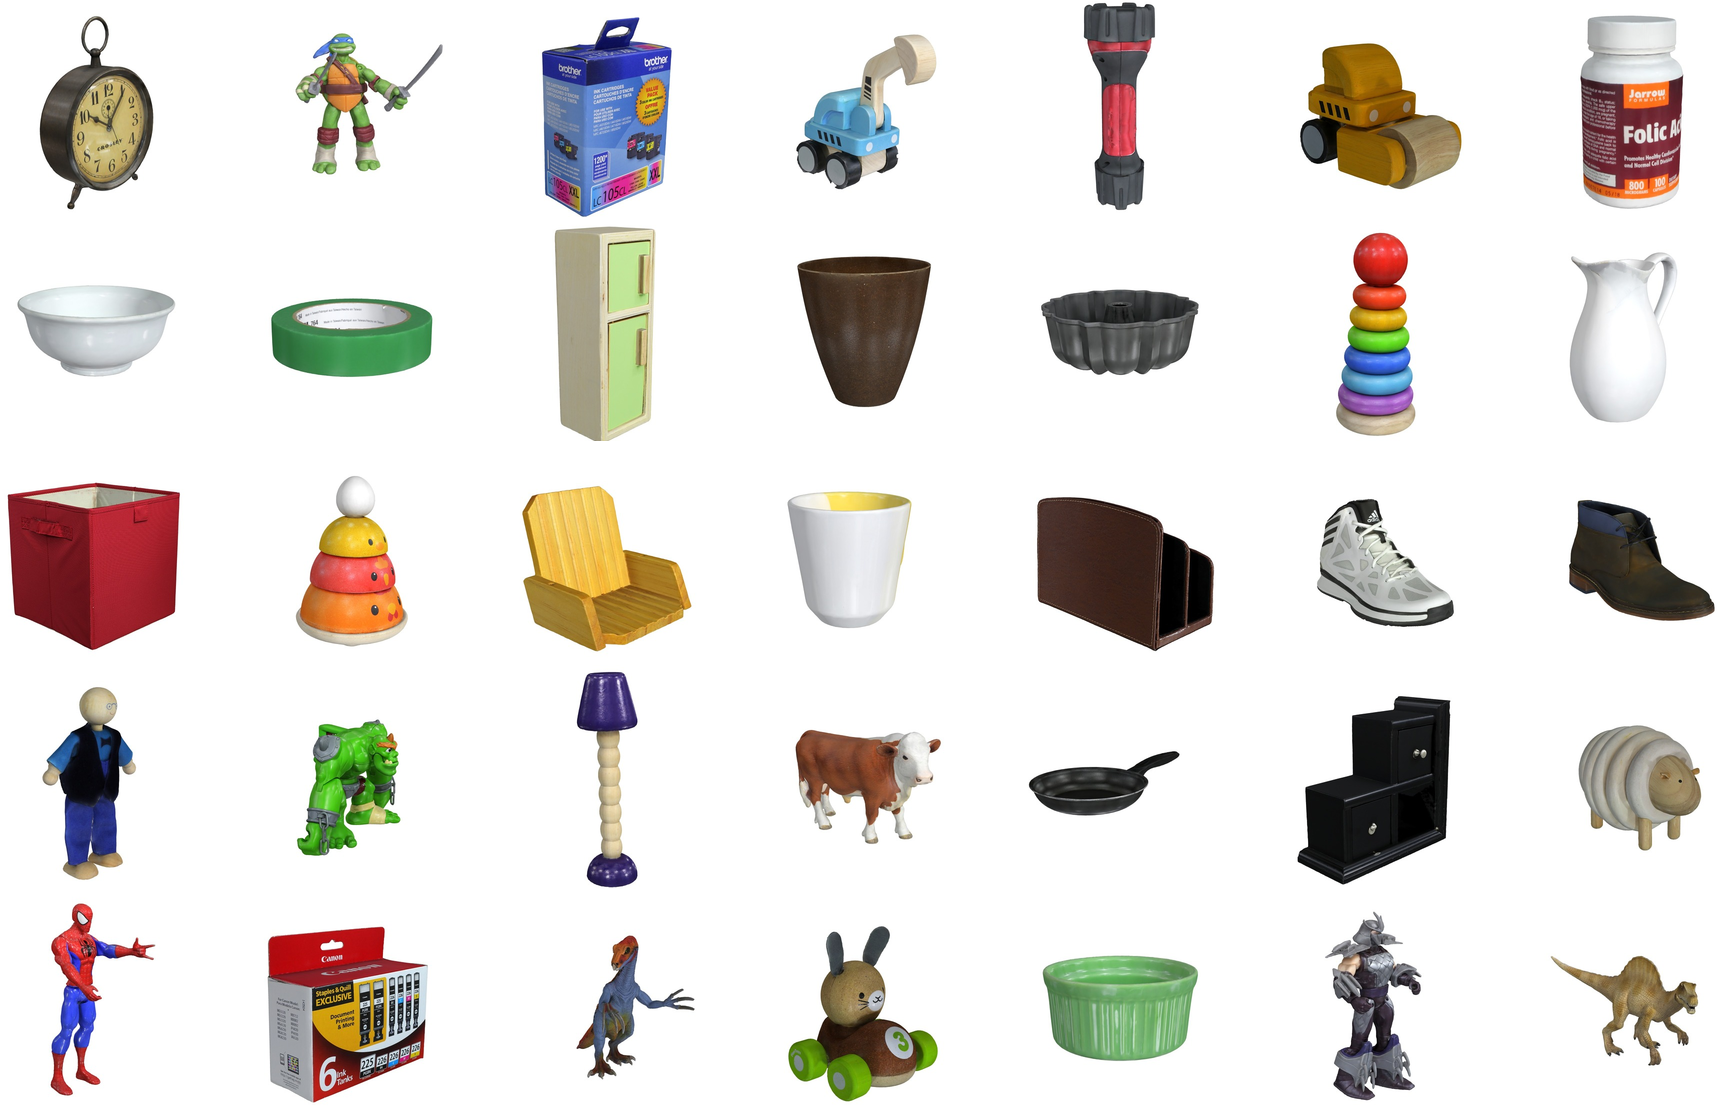
\includegraphics[height=4.75cm]{graphics/training_set.png}
        \end{column}
    \end{columns}
\end{frame}

\begin{frame}{Vision-Based Robotic Grasping of Diverse Objects}{Approach}
    \begin{columns}%
        \begin{column}{0.375\textwidth}%
            \begin{block}{Approaches}
                \begin{itemize}
                    \item Analytical
                    \item Empirical
                          \begin{itemize}
                              \item Supervised Learning
                              \item Imitation Learning
                              \item \only<1>{Reinforcement Learning}\only<2>{\textbf{Reinforcement Learning}}
                          \end{itemize}
                \end{itemize}
            \end{block}
        \end{column}
        %
        \begin{column}{0.625\textwidth}%
            \centering
            \onslide<2>{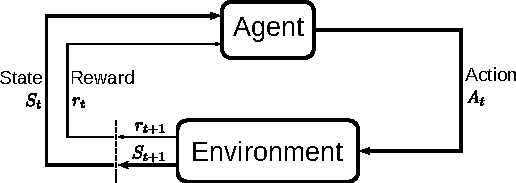
\includegraphics[width=\textwidth]{graphics/mdp_loop.pdf}}
        \end{column}
    \end{columns}
\end{frame}

\begin{frame}{Task Definition}{}
    \begin{columns}%
        \begin{column}{0.32\textwidth}%
            \begin{block}{Agent}
                \begin{itemize}
                    \item High-level controller
                          \begin{itemize}
                              \item Gripper pose
                              \item Gripper action
                          \end{itemize}
                \end{itemize}
            \end{block}
        \end{column}
        %
        \begin{column}{0.32\textwidth}%
            \begin{block}{Environment}
                \begin{itemize}
                    \item Objects
                    \item Robot
                          \begin{itemize}
                              \item Low-level controllers
                          \end{itemize}
                    \item Physics and visuals
                \end{itemize}
            \end{block}
        \end{column}
        %
        \begin{column}{0.35\textwidth}%
            \begin{block}{Episodic Task}
                \begin{itemize}
                    \item Success
                          \begin{itemize}
                              \item Lifting an object
                          \end{itemize}
                    \item Failure
                          \begin{itemize}
                              \item Pushing all objects away
                          \end{itemize}
                    \item Max 100 time steps
                          \begin{itemize}
                              \item \textasciitilde 40 s (simulation)
                          \end{itemize}
                \end{itemize}
            \end{block}
        \end{column}
    \end{columns}
\end{frame}

\begin{frame}{Action Space}{}
    \begin{columns}%
        \begin{column}{0.4\textwidth}%
            \begin{block}{Actions in Cartesian space}
                \begin{itemize}
                    \item Translational displacement
                          \begin{itemize}
                              \item \(d_{x}\)
                              \item \(d_{y}\)
                              \item \(d_{z}\)
                          \end{itemize}
                    \item Gripper rotation
                          \begin{itemize}
                              \item \(d_{\phi}\)
                          \end{itemize}
                    \item Gripper actions (open/close)
                          \begin{itemize}
                              \item \(g\)
                          \end{itemize}
                \end{itemize}
            \end{block}
        \end{column}
        %
        \begin{column}{0.6\textwidth}%
            \centering
            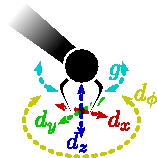
\includegraphics[height=6cm]{graphics/action_space.pdf}
        \end{column}
    \end{columns}
\end{frame}

\begin{frame}{Observation Space}{}
    \begin{columns}%
        \begin{column}{0.6\textwidth}%
            \centering
            \only<1>{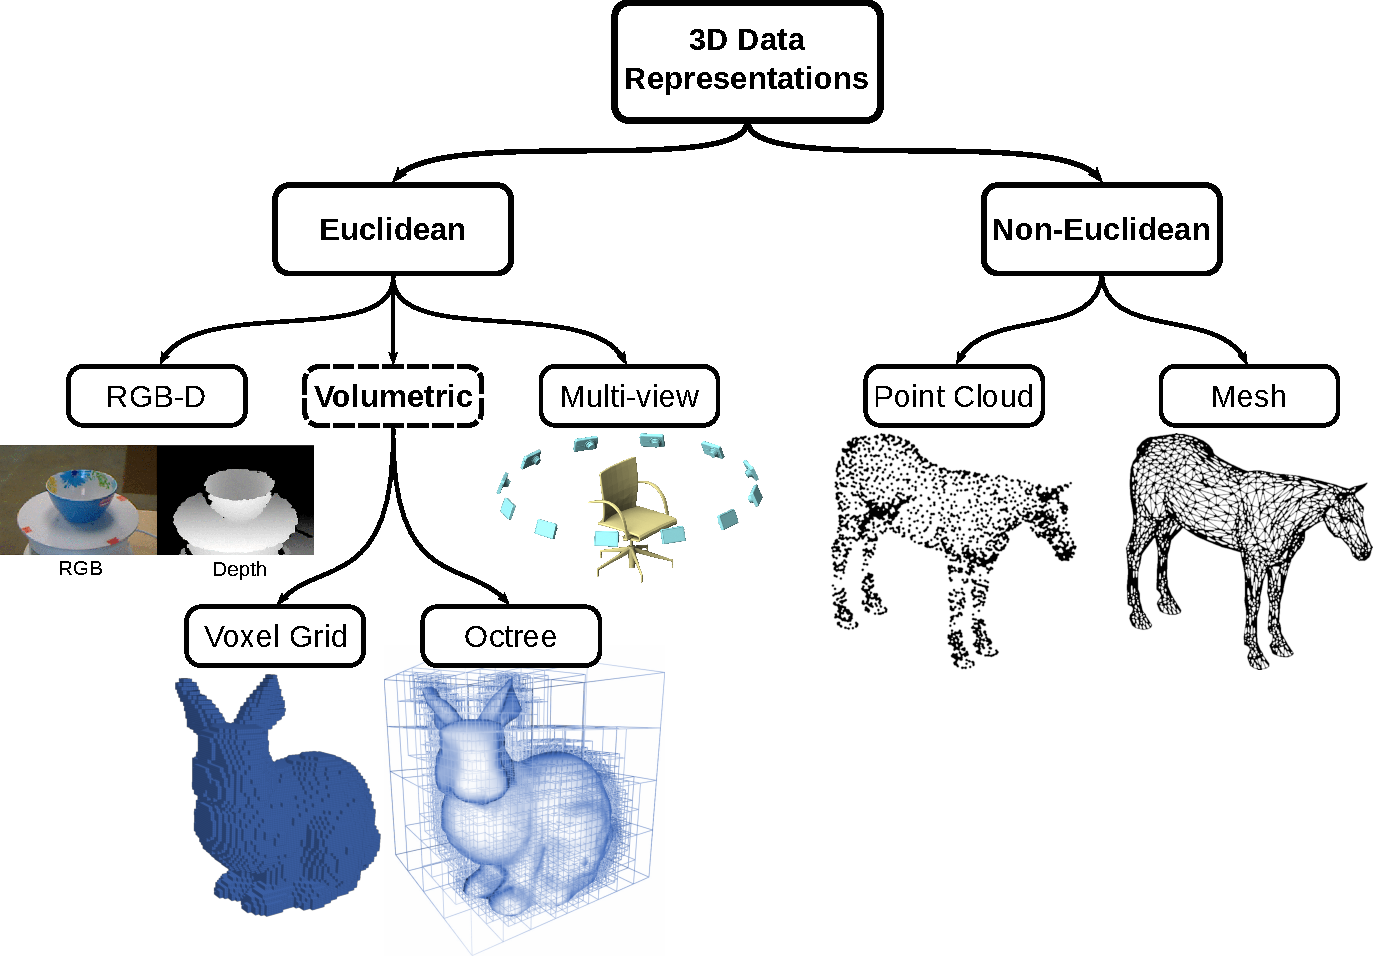
\includegraphics[height=6.5cm]{graphics/3d_data_representations.pdf}}\only<2->{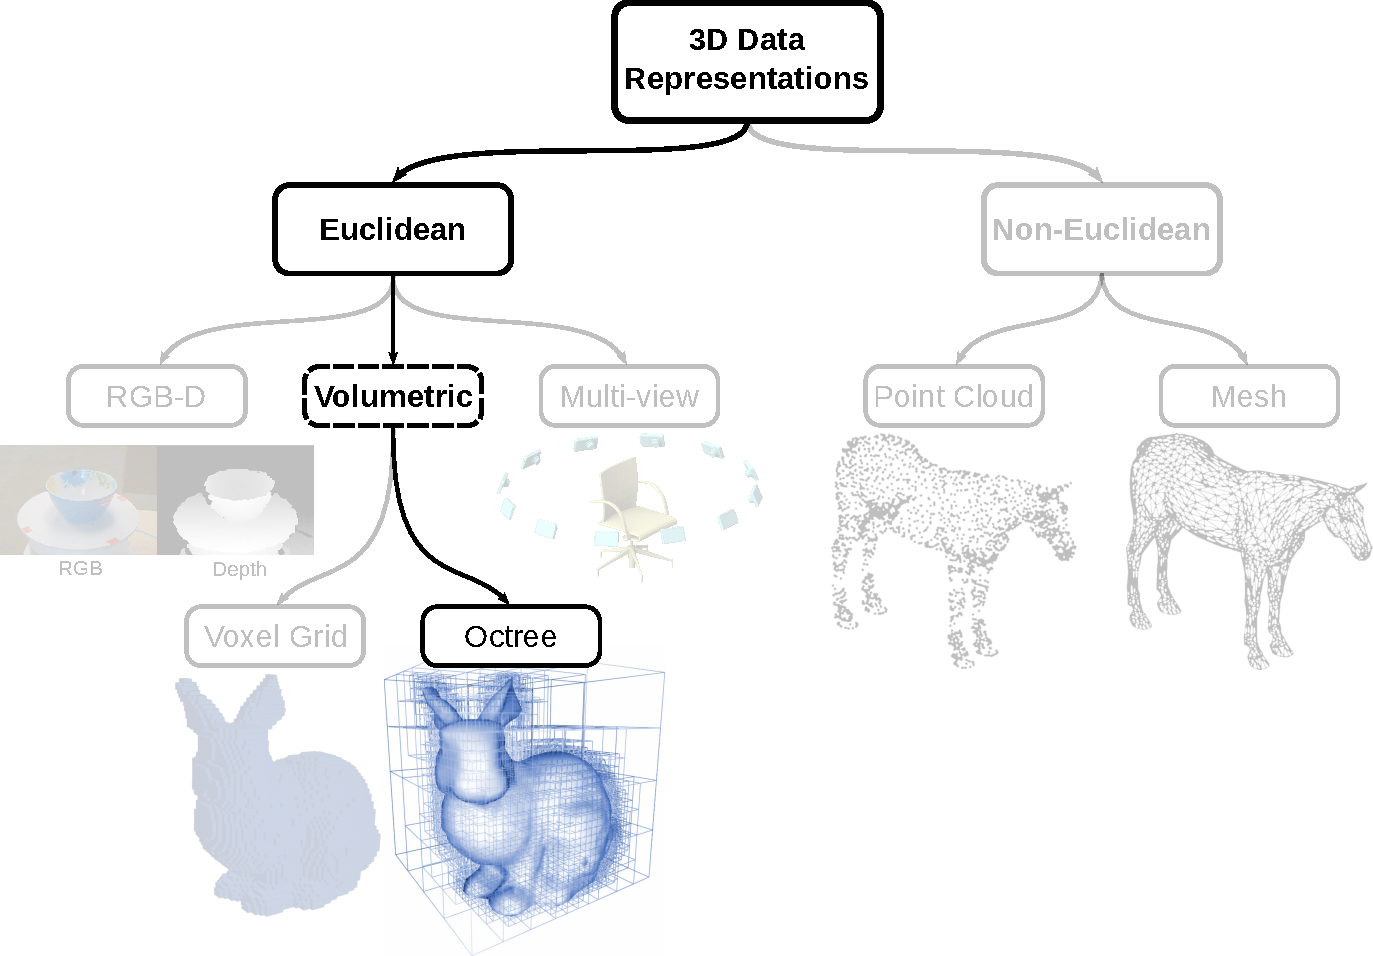
\includegraphics[height=6.5cm]{graphics/3d_data_representations_only_octree.pdf}}
        \end{column}
        %
        \begin{column}{0.4\textwidth}%
            \onslide<3>{
                \begin{block}{Proprioceptive Observations}
                    \begin{itemize}
                        \item Gripper position
                        \item Gripper rotation
                        \item Gripper state
                    \end{itemize}
                \end{block}
            }
        \end{column}
    \end{columns}
    \only<1>{\footnoteref{}}\only<2->{\footnoteref{Wang et al. 2017. O-CNN: Octree-based Convolutional Neural Networks for 3D Shape Analysis. ACM Trans. Graph. (SIGGRAPH) 36, 4, Article 72.}}
\end{frame}

\begin{frame}{Observation Space}{Construction of Octree}
    \centering
    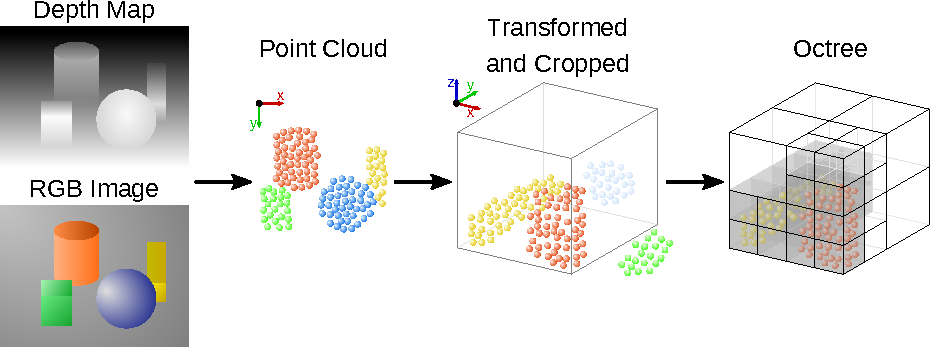
\includegraphics[width=\textwidth]{graphics/octree_creation_sketch.pdf}
\end{frame}

\begin{frame}{Observation Space}{Features and Stacks}
    \begin{columns}%
        \begin{column}{0.5\textwidth}%
            \begin{block}{Features}
                \begin{itemize}
                    \item Spatial
                          \begin{itemize}
                              \item Average normal vector \(\overline{n}\)
                              \item Average distance to points \(\overline{d}\)
                          \end{itemize}
                    \item Colour
                          \begin{itemize}
                              \item Average intensity of RGB channels \(\overline{rgb}\)
                          \end{itemize}
                \end{itemize}
            \end{block}
            \begin{block}{Observation Stacking}
                \begin{itemize}
                    \item Three consecutive stacks
                \end{itemize}
            \end{block}
        \end{column}
        %
        \begin{column}{0.5\textwidth}%
            \centering
            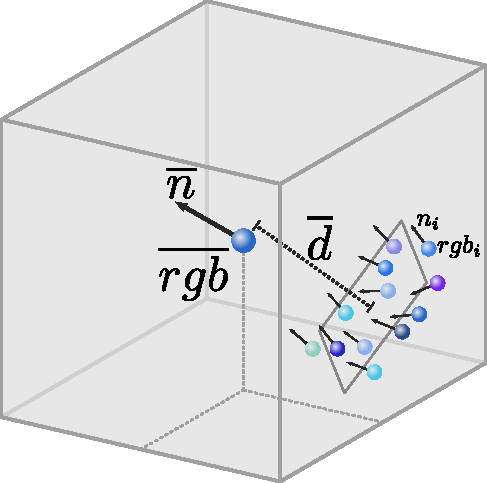
\includegraphics[height=5cm]{graphics/octree_features_sketch.pdf}
        \end{column}
    \end{columns}
\end{frame}

\begin{frame}{Reward Function}{}
    \begin{columns}%
        \begin{column}{0.5\textwidth}%
            \begin{block}{Composite Reward}
                \begin{itemize}
                    \item Reach
                          \begin{itemize}
                              \item \(+1\) (\(7^{0}\))
                          \end{itemize}
                    \item Touch
                          \begin{itemize}
                              \item \(+7\) (\(7^{1}\))
                          \end{itemize}
                    \item Grasp
                          \begin{itemize}
                              \item \(+49\) (\(7^{2}\))
                          \end{itemize}
                    \item Lift
                          \begin{itemize}
                              \item \(+343\) (\(7^{3}\))
                          \end{itemize}
                \end{itemize}
            \end{block}
        \end{column}
        %
        \begin{column}{0.5\textwidth}%
            \begin{block}{Recurring Reward}
                \begin{itemize}
                    \item Collision with ground/table
                          \begin{itemize}
                              \item \(-1\)
                          \end{itemize}
                    \item Incentive to act quickly
                          \begin{itemize}
                              \item \(-0.005\)
                          \end{itemize}
                \end{itemize}
            \end{block}
        \end{column}
    \end{columns}
\end{frame}

\begin{frame}{Reinforcement Learning}{Algorithms}
    \begin{columns}%
        \begin{column}{0.3\textwidth}%
            \begin{block}{Actor-Critic Algorithms}
                \begin{itemize}
                    \item TD3
                    \item SAC
                    \item TQC
                \end{itemize}
            \end{block}
            \begin{block}{Implementation}
                \begin{itemize}
                    \item Stable Baselines3
                \end{itemize}
            \end{block}
        \end{column}
        %
        \begin{column}{0.7\textwidth}%
            \centering
            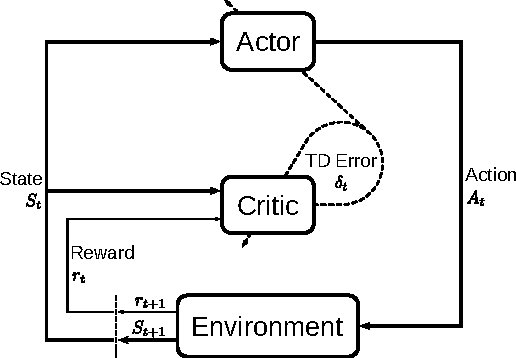
\includegraphics[height=6cm]{graphics/actor_critic_loop.pdf}
        \end{column}
    \end{columns}
\end{frame}

\begin{frame}{Deep Reinforcement Learning}{Octree-Based Feature Extractor}
    \centering
    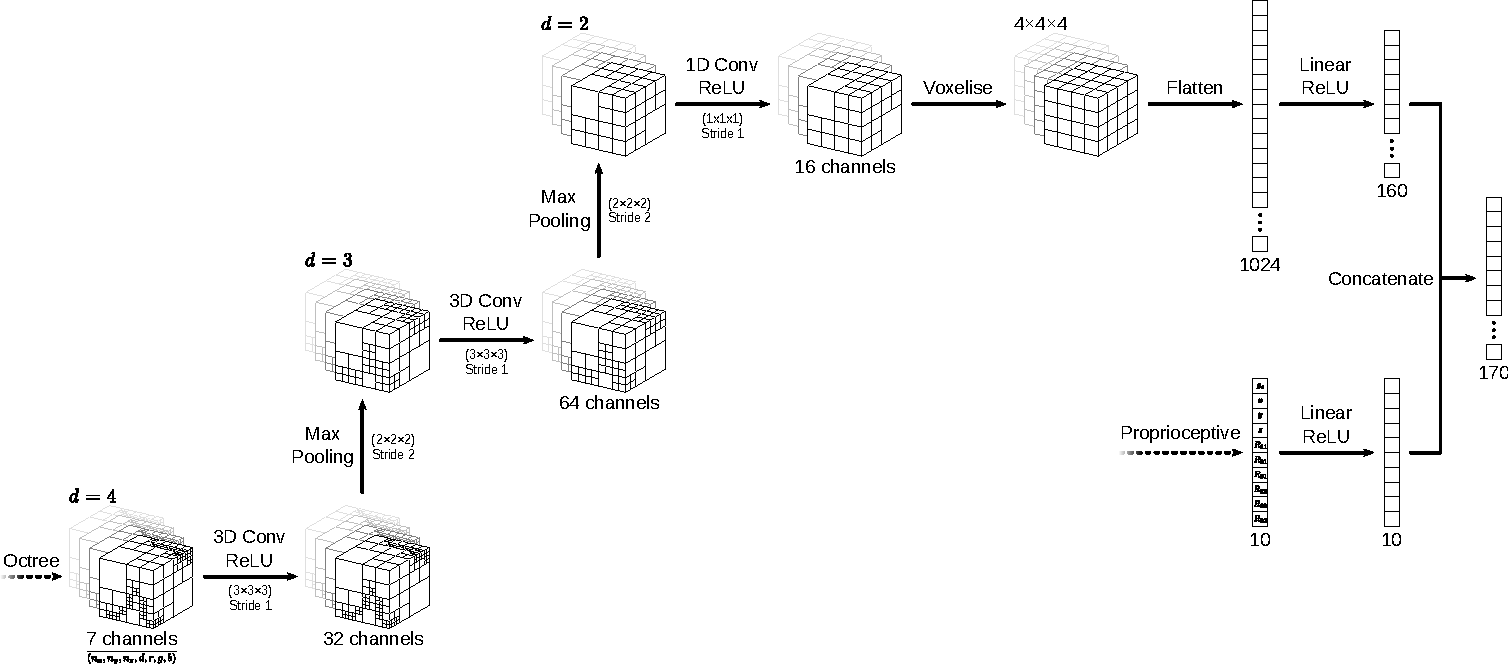
\includegraphics[width=\textwidth]{graphics/feature_extractor.pdf}
\end{frame}

\begin{frame}{Deep Reinforcement Learning}{Full Actor-Critic Network Architecture}
    \centering
    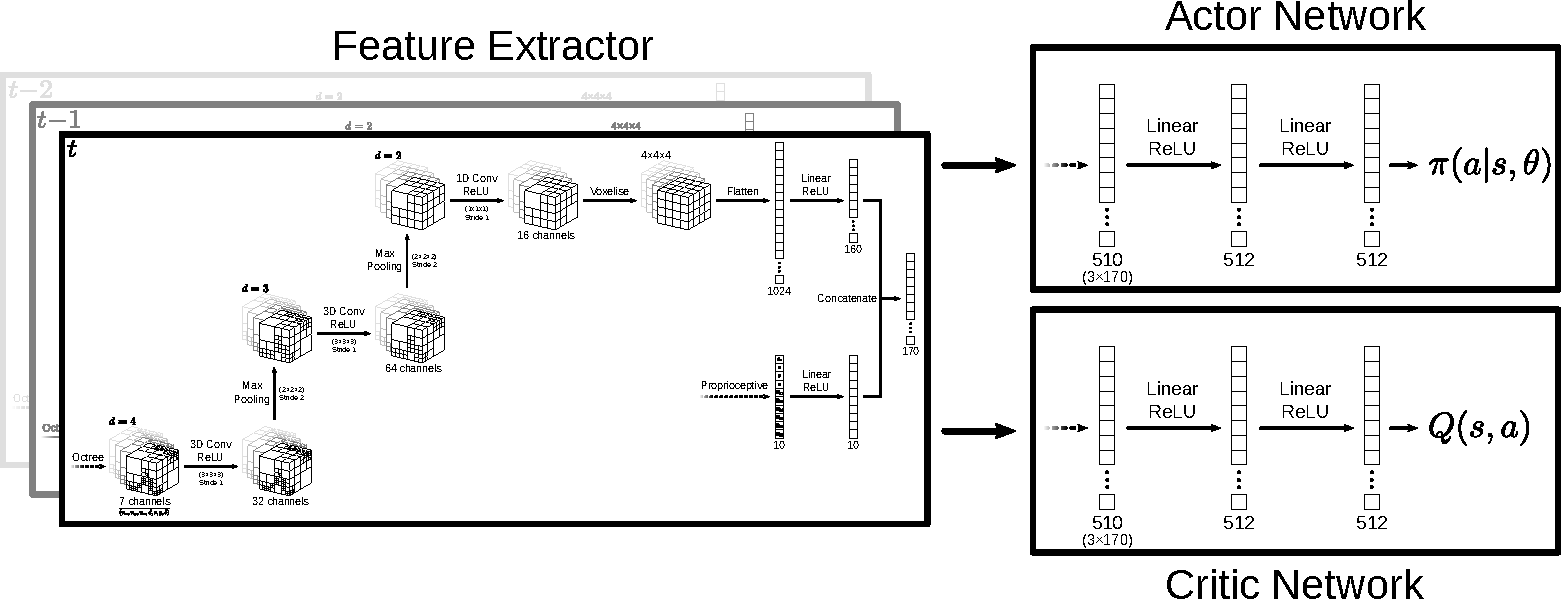
\includegraphics[width=\textwidth]{graphics/actor_critic_network_full.pdf}
\end{frame}



